\documentclass[10pt]{article}
\usepackage[margin=0.48in]{geometry}
\usepackage[T1]{fontenc}
\usepackage{newtxtext,newtxmath}
\usepackage{microtype}
\usepackage{amsmath,mathtools,booktabs,array,graphicx}
\usepackage[most]{tcolorbox}
\usepackage{xcolor}
\usepackage{multicol}
\usepackage{tikz}
\usetikzlibrary{arrows.meta,calc,positioning}
\usepackage[hidelinks]{hyperref}

\pagestyle{empty}
\setlength{\parindent}{0pt}
\setlength{\parskip}{2.8pt}
\setlength{\columnsep}{16pt}
\linespread{0.98}
\AtBeginEnvironment{multicols}{\small}
\raggedcolumns
\renewcommand{\arraystretch}{1.08}

\definecolor{ink}{HTML}{15364C}
\definecolor{accent}{HTML}{0F6E9D}
\definecolor{soft}{HTML}{EEF6FB}
\definecolor{softline}{HTML}{B7D4E5}
\definecolor{softgray}{HTML}{F4F7F9}
\definecolor{grayline}{HTML}{D5DEE5}
\definecolor{hamlight}{HTML}{F4F7F9}
\definecolor{qbg}{HTML}{EEF3F7}
\definecolor{pbg}{HTML}{F4F0EC}
\definecolor{qline}{HTML}{7F96A6}
\definecolor{pline}{HTML}{AD8F7B}
\definecolor{regbg}{HTML}{EEF6FB}
\definecolor{goldbg}{HTML}{F5F2E8}
\definecolor{goldline}{HTML}{B59A62}
\definecolor{regline}{HTML}{9BB9CA}

\newtcolorbox{keybox}{
  enhanced,
  colback=soft,
  colframe=softline,
  boxrule=0.5pt,
  arc=1.4mm,
  left=7pt,right=7pt,top=6pt,bottom=6pt
}

\newtcolorbox{takebox}{
  enhanced,
  colback=softgray,
  colframe=grayline,
  boxrule=0.5pt,
  arc=1.2mm,
  left=7pt,right=7pt,top=5pt,bottom=5pt
}

\newcommand{\hm}[1]{\ensuremath{#1}}

\tikzset{
  hambox/.style={draw=black!48, rounded corners=2pt, line width=0.75pt, fill=white, align=center, inner sep=2.2pt, font=\small},
  hamsmall/.style={draw=black!42, rounded corners=2pt, line width=0.65pt, fill=white, align=center, inner sep=2pt, font=\footnotesize},
  hammath/.style={font=\small},
  hamgroup/.style={draw=grayline!90!black, rounded corners=2.4pt, line width=0.75pt},
  hamarrow/.style={-{Latex[length=2.6mm,width=2.0mm]}, line width=0.95pt, draw=black!65},
  hamsoftarrow/.style={-{Latex[length=2.3mm,width=1.8mm]}, line width=0.85pt, draw=black!48},
  qfill/.style={draw=qline, fill=qbg},
  pfill/.style={draw=pline, fill=pbg},
  regfill/.style={draw=regline, fill=regbg},
  goldfill/.style={draw=goldline, fill=goldbg}
}

\begin{document}

{\Large\bfseries\color{ink} Beyond Isotropy in JEPAs: Hamiltonian Geometry and Symplectic Prediction}\par
{\small\color{accent}\textbf{Technical summary}}\par\vspace{3pt}

\begin{keybox}
\textbf{Core idea.} The paper's central reframing is that Euclidean isotropy is \emph{not} a neutral regularizer. It is already a metric choice. If downstream tasks live in a structured geometry encoded by an SPD operator \(H\succ0\), then the canonical representation is not ``round in ambient coordinates'' but round only \emph{after whitening by} \(H^{1/2}\). Under an \(H\)-energy budget, both the minimax covariance and the maximum-entropy law are proportional to \(H^{-1}\), and forcing \(\Sigma\propto I\) incurs a closed-form price of isotropy.
\end{keybox}

\vspace{2pt}
\begin{center}
\resizebox{0.78\textwidth}{!}{%
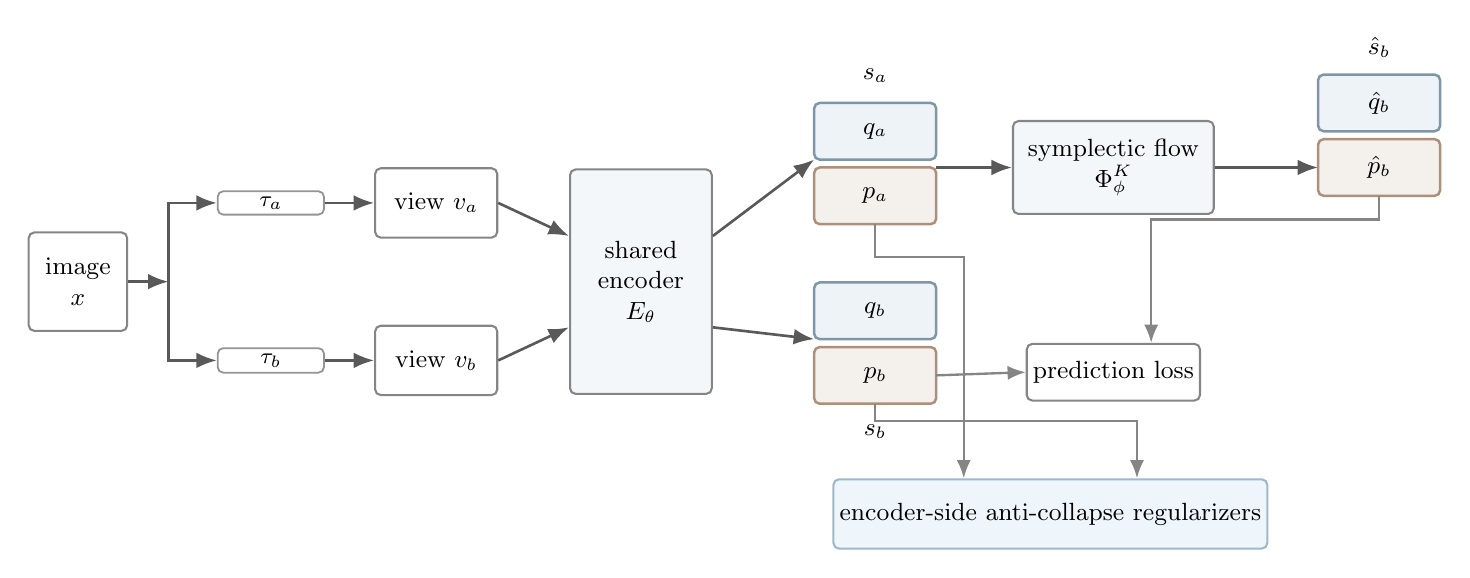
\begin{tikzpicture}[x=1cm,y=1cm]

  % nodes
  \node[hambox, minimum width=1.25cm, minimum height=1.25cm] (img) at (0,0) {image\\$x$};
  \coordinate (branch) at (1.15,0);

  \node[hamsmall, minimum width=1.35cm] (taua) at (2.45,1.0) {$\tau_a$};
  \node[hamsmall, minimum width=1.35cm] (taub) at (2.45,-1.0) {$\tau_b$};

  \node[hambox, minimum width=1.55cm, minimum height=0.88cm] (va) at (4.55,1.0) {view $v_a$};
  \node[hambox, minimum width=1.55cm, minimum height=0.88cm] (vb) at (4.55,-1.0) {view $v_b$};

  \node[hambox, minimum width=1.8cm, minimum height=2.85cm, fill=hamlight] (enc) at (7.15,0) {shared\\encoder\\$E_\theta$};

  % s_a
  \draw[qfill, rounded corners=2pt, line width=0.9pt] (9.35,1.55) rectangle +(1.55,0.72);
  \draw[pfill, rounded corners=2pt, line width=0.9pt] (9.35,0.73) rectangle +(1.55,0.72);
  \node[hammath] at (10.125,1.91) {\hm{q_a}};
  \node[hammath] at (10.125,1.09) {\hm{p_a}};
  \node[hammath] at (10.125,2.62) {\hm{s_a}};

  % s_b
  \draw[qfill, rounded corners=2pt, line width=0.9pt] (9.35,-0.73) rectangle +(1.55,0.72);
  \draw[pfill, rounded corners=2pt, line width=0.9pt] (9.35,-1.55) rectangle +(1.55,0.72);
  \node[hammath] at (10.125,-0.37) {\hm{q_b}};
  \node[hammath] at (10.125,-1.19) {\hm{p_b}};
  \node[hammath] at (10.125,-1.90) {\hm{s_b}};

  % flow
  \node[hambox, minimum width=2.55cm, minimum height=1.18cm, fill=hamlight] (flow) at (13.15,1.45) {symplectic flow\\\hm{\Phi_\phi^{K}}};

  % s_hat_b
  \draw[qfill, rounded corners=2pt, line width=0.9pt] (15.75,1.91) rectangle +(1.55,0.72);
  \draw[pfill, rounded corners=2pt, line width=0.9pt] (15.75,1.09) rectangle +(1.55,0.72);
  \node[hammath] at (16.525,2.27) {\hm{\hat q_b}};
  \node[hammath] at (16.525,1.45) {\hm{\hat p_b}};
  \node[hammath] at (16.525,2.98) {\hm{\hat s_b}};

  % comparison + regularizers
  \node[hambox, minimum width=2.15cm, minimum height=0.72cm] (loss) at (13.15,-1.15) {prediction loss};
  \node[hambox, regfill, minimum width=4.9cm, minimum height=0.88cm] (regs) at (12.35,-2.95) {encoder-side anti-collapse regularizers};

  % routing coordinates
  \coordinate (saeast)   at (10.90,1.45);
  \coordinate (sbout)    at (10.90,-1.19);   % right edge of p_b box
  \coordinate (shatleft) at (15.75,1.45);
  \coordinate (shatdown) at (16.525,1.09);

  \coordinate (lossL) at ($(loss.north)+(-0.48,0)$);
  \coordinate (lossR) at ($(loss.north)+(0.48,0)$);

  \coordinate (regL) at ($(regs.north)+(-1.10,0)$);
  \coordinate (regR) at ($(regs.north)+(1.10,0)$);

  % arrows: left side
  \draw[hamarrow] (img.east) -- (branch);
  \draw[hamarrow] (branch) |- (taua.west);
  \draw[hamarrow] (branch) |- (taub.west);

  \draw[hamarrow] (taua.east) -- (va.west);
  \draw[hamarrow] (taub.east) -- (vb.west);

  \draw[hamarrow] (va.east) -- ($(enc.west)+(0,0.58)$);
  \draw[hamarrow] (vb.east) -- ($(enc.west)+(0,-0.58)$);

  \draw[hamarrow] ($(enc.east)+(0,0.58)$) -- (9.35,1.55);
  \draw[hamarrow] ($(enc.east)+(0,-0.58)$) -- (9.35,-0.73);

  % arrows: right side
  \draw[hamarrow] (saeast) -- (flow.west);
  \draw[hamarrow] (flow.east) -- (shatleft);

  % fixed loss arrows
  \draw[hamsoftarrow] (sbout) -- (loss.west);
  \draw[hamsoftarrow] (shatdown) -- ++(0,-0.30) -| (lossR);

  % regularizer arrows
  \draw[hamsoftarrow] (10.125,0.73)  -- ++(0,-0.42) -| (regL);
  \draw[hamsoftarrow] (10.125,-1.55) -- ++(0,-0.22) -| (regR);

\end{tikzpicture}%
}
\end{center}

\vspace{-1pt}
\begin{takebox}
\textbf{Reported downstream results (all q / p / \((q,p)\) readouts that the paper reports explicitly).}\vspace{3pt}

\begin{minipage}[t]{0.49\textwidth}
\centering\scriptsize
\textbf{CIFAR-100, 30 epochs}\par\vspace{2pt}
\begin{tabular}{@{}lcc@{}}
\toprule
Method & kNN@20 & Linear \\
\midrule
SIGReg & $26.56\pm0.18$ & $30.43\pm0.30$ \\
HamJEPA $q$ & $31.45\pm0.27$ & $33.95\pm0.24$ \\
HamJEPA $p$ & $29.71\pm0.25$ & $33.07\pm0.36$ \\
HamJEPA $(q,p)$ & $30.88\pm0.39$ & $34.18\pm0.17$ \\
\bottomrule
\end{tabular}
\end{minipage}\hfill
\begin{minipage}[t]{0.49\textwidth}
\centering\scriptsize
\textbf{ImageNet-100, 45 epochs}\par\vspace{2pt}
\begin{tabular}{@{}lcc@{}}
\toprule
Method & kNN@20 & Linear \\
\midrule
SIGReg $q$ & $20.10$ & $24.40$ \\
SIGReg $p$ & $18.78$ & $23.86$ \\
SIGReg $(q,p)$ & $20.94$ & $25.54$ \\
HamJEPA $q$ & $24.92$ & $31.92$ \\
HamJEPA $p$ & $24.72$ & $32.08$ \\
HamJEPA $(q,p)$ & $24.64$ & $32.04$ \\
\bottomrule
\end{tabular}
\end{minipage}

\vspace{5pt}
\centering\scriptsize
\textbf{CIFAR-100, 80 epochs: predictor-family ablation}\par\vspace{2pt}
\begin{tabular}{@{}llccc@{}}
\toprule
Method & Variant & Linear & kNN@20 & kNN best \\
\midrule
SIGReg & single & $33.95$ & $27.98$ & $28.71\ @\ k=1$ \\
MLP-HJEPA & $q$ & $42.26$ & $28.10$ & $28.10\ @\ k=20$ \\
MLP-HJEPA & $p$ & $41.90$ & $28.30$ & $28.30\ @\ k=20$ \\
MLP-HJEPA & $(q,p)$ & $42.77$ & $28.15$ & $28.15\ @\ k=20$ \\
HamJEPA & $q$ & $44.59$ & $34.43$ & $34.43\ @\ k=20$ \\
HamJEPA & $p$ & $44.44$ & $32.96$ & $32.96\ @\ k=20$ \\
HamJEPA & $(q,p)$ & $44.52$ & $33.66$ & $33.66\ @\ k=20$ \\
\bottomrule
\end{tabular}

\vspace{3pt}
{\scriptsize\emph{Note.} The paper's main 30-epoch CIFAR table reports SIGReg only as a single baseline; the explicit q/p/\((q,p)\) decomposition is reported there for HamJEPA, for both methods on ImageNet-100, and for both HamJEPA and the non-symplectic MLP-HJEPA ablation at 80 epochs.}
\end{takebox}

\vspace{4pt}
\begin{multicols}{2}

\textbf{\color{ink}1. The main theoretical move.} A lot of JEPA work regularizes toward an isotropic Gaussian because isotropy feels like a generic anti-collapse prior. This paper says that instinct is already doing something much stronger: it is declaring the ambient Euclidean metric to be the correct notion of symmetry. If the downstream task family has structure, that is the wrong reference frame. The right question is not ``should the latent be spherical?'' It is ``spherical with respect to \emph{which} metric?''

The theory formalizes that point by introducing a structured SPD operator \(H\succ0\), modeling downstream linear tasks by
\[
y=w^\top \tilde z,\qquad \mathcal W_H=\{w: w^\top H^{-1}w\le 1\},
\]
and imposing an \(H\)-energy budget
\[
\operatorname{tr}(H\Sigma)=c,\qquad \Sigma=\operatorname{Cov}(\tilde z).
\]
Under that geometry, the unique minimax covariance is
\[
\Sigma^\star=\frac{c}{d}H^{-1},
\]
and the unique maximum-entropy law under the same constraint is
\[
\tilde z\sim \mathcal N\!\left(0,\frac{c}{d}H^{-1}\right).
\]
So the canonical object is anisotropic in the original coordinates and isotropic only after whitening by \(H^{1/2}\).

\textbf{\color{ink}2. The price of using the wrong sphere.} If one nevertheless insists on Euclidean isotropy, the only feasible covariance under the same budget is
\[
\Sigma_{\mathrm{iso}}=\frac{c}{\operatorname{tr}(H)}I,
\]
and the worst-case task variance degrades by
\[
\rho(H)=\frac{V(\Sigma_{\mathrm{iso}})}{V(\Sigma^\star)}
=\frac{d\,\lambda_{\max}(H)}{\operatorname{tr}(H)},
\qquad 1\le \rho(H)\le d.
\]
That formula is the paper's cleanest insight. ``Isotropic'' is only optimal when the task geometry itself is Euclidean, i.e. when \(H\propto I\). Otherwise Euclidean isotropy is not unbiased regularization; it is a mismatch penalty.

A useful bridge to the architecture is the phase-space lift of this structured Gaussian. With
\[
\mathcal H_H(q,p)=\tfrac12 q^\top Hq+\tfrac12\|p\|_2^2,
\qquad
\pi_H(q,p)\propto \exp\!\Bigl(-\frac{d}{c}\mathcal H_H(q,p)\Bigr),
\]
the \(q\)-marginal is exactly \(\mathcal N(0,(c/d)H^{-1})\) while \(p\sim \mathcal N(0,(c/d)I)\). The paper's practical move is then: if the right geometry is phase-space-like, put structure in the transport map rather than forcing a Euclidean sphere at the encoder output.

\textbf{\color{ink}3. What HamJEPA actually changes.} Because the relevant \(H\) is unknown in practice, the method does not hard-code a structured encoder marginal. Instead it places Hamiltonian structure in the \emph{predictor}. Each view is encoded as a phase-space state \(s=(q,p)\), where \(q\) is the intended content coordinate and \(p\) is an auxiliary momentum-like state. Cross-view prediction is then done by a \(K\)-step leapfrog rollout of a separable Hamiltonian
\[
\mathcal H_\phi(q,p)=\tfrac12\|p\|_2^2+V_\phi(q).
\]
The resulting predictor map \(\hat s_b=\Phi_\phi^K(s_a)\) is symplectic, volume-preserving, and exactly reversible under time-step sign reversal. The important claim is not that the encoder itself becomes Hamiltonian in any literal physical sense; it is that the view-to-view predictor can no longer be an arbitrary geometry-destroying regressor.

\textbf{\color{ink}4. Symplecticity is not the same thing as anti-collapse.} The paper is careful about this. A symplectic predictor cannot locally crush phase-space volume, but the encoder could still emit a degenerate state cloud. HamJEPA therefore adds encoder-side non-collapse terms: fixed-unit energy budgets for \(q\) and \(p\), a projected log-determinant floor, and a participation-ratio floor. These are deliberately weaker and more geometry-aware than forcing \(\Sigma\propto I\): they preserve scale and rank without declaring all directions equivalent.

\end{multicols}

\vspace{-2pt}
\begin{center}
\resizebox{0.72\textwidth}{!}{%
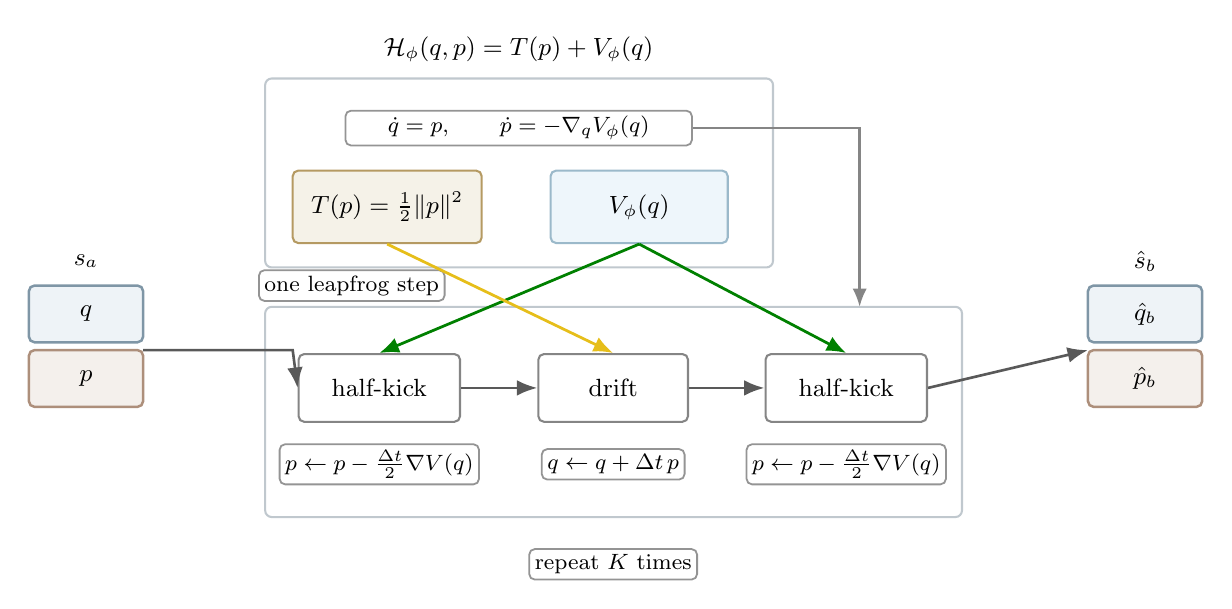
\begin{tikzpicture}[x=1cm,y=1cm]

  % input state
  \draw[qfill, rounded corners=2pt, line width=0.9pt] (0.0,1.0) rectangle +(1.45,0.72);
  \draw[pfill, rounded corners=2pt, line width=0.9pt] (0.0,0.18) rectangle +(1.45,0.72);
  \node[hammath] at (0.725,1.36) {\hm{q}};
  \node[hammath] at (0.725,0.54) {\hm{p}};
  \node[hammath] at (0.725,2.03) {\hm{s_a}};

  % Hamiltonian group
  \draw[hamgroup] (3.0,1.95) rectangle (9.45,4.35);
  \node[hammath] at (6.22,4.72) {\hm{\mathcal H_\phi(q,p)=T(p)+V_\phi(q)}};

  \node[hamsmall, minimum width=4.4cm] (dyn) at (6.22,3.72)
  {\hm{\dot q=p,\qquad \dot p=-\nabla_q V_\phi(q)}};

  \node[hambox, goldfill, minimum width=2.4cm, minimum height=0.92cm] (Tbox) at (4.55,2.72)
  {\hm{T(p)=\tfrac12\|p\|^2}};
  \node[hambox, regfill, minimum width=2.25cm, minimum height=0.92cm] (Vbox) at (7.75,2.72)
  {\hm{V_\phi(q)}};

  % leapfrog group
  \draw[hamgroup] (3.0,-1.22) rectangle (11.85,1.45);
  \node[hamsmall, fill=white, inner sep=2pt] at (4.10,1.72) {one leapfrog step};

  \node[hambox, minimum width=2.05cm, minimum height=0.86cm] (kick1) at (4.45,0.42) {half-kick};
  \node[hambox, minimum width=1.90cm, minimum height=0.86cm] (drift) at (7.42,0.42) {drift};
  \node[hambox, minimum width=2.05cm, minimum height=0.86cm] (kick2) at (10.38,0.42) {half-kick};

  \node[hamsmall] at (4.45,-0.55) {\hm{p\leftarrow p-\tfrac{\Delta t}{2}\nabla V(q)}};
  \node[hamsmall] at (7.42,-0.55) {\hm{q\leftarrow q+\Delta t\,p}};
  \node[hamsmall] at (10.38,-0.55) {\hm{p\leftarrow p-\tfrac{\Delta t}{2}\nabla V(q)}};

  \node[hamsmall, minimum width=2.0cm] at (7.42,-1.82) {repeat $K$ times};

  % output
  \draw[qfill, rounded corners=2pt, line width=0.9pt] (13.45,1.0) rectangle +(1.45,0.72);
  \draw[pfill, rounded corners=2pt, line width=0.9pt] (13.45,0.18) rectangle +(1.45,0.72);
  \node[hammath] at (14.175,1.36) {\hm{\hat q_b}};
  \node[hammath] at (14.175,0.54) {\hm{\hat p_b}};
  \node[hammath] at (14.175,2.03) {\hm{\hat s_b}};

  % arrows through predictor
  \draw[hamarrow] (1.45,0.90) -- (3.35,0.90) -- (kick1.west);
  \draw[hamarrow] (kick1.east) -- (drift.west);
  \draw[hamarrow] (drift.east) -- (kick2.west);
  \draw[hamarrow] (kick2.east) -- (13.45,0.90);

  % straight dependency arrows to top-midpoints of the small boxes
  \draw[-{Latex[length=2.5mm,width=2mm]}, line width=1.0pt, draw=green!50!black]
    (Vbox.south) -- (kick1.north);
  \draw[-{Latex[length=2.5mm,width=2mm]}, line width=1.0pt, draw=green!50!black]
    (Vbox.south) -- (kick2.north);
  \draw[-{Latex[length=2.5mm,width=2mm]}, line width=1.0pt, draw=yellow!65!orange!90!black]
    (Tbox.south) -- (drift.north);

  % dynamics arrow: right, then straight down to the top edge of the gray box
  \coordinate (dynelbow) at (10.55,3.72);
  \coordinate (dynhook)  at (10.55,1.45);
  \draw[hamsoftarrow] (dyn.east) -- (dynelbow) -- (dynhook);

\end{tikzpicture}%
}
\end{center}

\vspace{0pt}
\begin{multicols}{2}

\textbf{\color{ink}5. What is held fixed, and why that matters.} The comparisons are deliberately controlled. Across methods, the paper keeps the JEPA backbone, augmentations, optimizer, batch size, and training schedule fixed; both datasets use a headless token regime based on ResNet stage-3 features, and the projector is the identity map so that the \(q/p\) split is not remixed away by an MLP head. This is why the results should be read as a geometry argument rather than a recipe argument.

\textbf{\color{ink}6. How to read the q/p results.} On CIFAR-100 at 30 epochs, \(q\) is the strongest HamJEPA readout for kNN, while \((q,p)\) gives the best linear probe. The intended interpretation is that \(q\) carries the cleanest metric-consistent content geometry, whereas \(p\) carries complementary linearly decodable signal that helps a learned probe more than raw nearest-neighbor structure. On ImageNet-100 the picture changes because the stable regime matches the full state \((q,p)\) during pretraining. There, \(q\), \(p\), and \((q,p)\) are all strong and nearly tied for HamJEPA, while for SIGReg the concatenated \((q,p)\) readout remains better than either half alone. The paper reads that difference as complementarity for SIGReg versus redundancy for HamJEPA: HamJEPA makes both coordinates individually informative.

\textbf{\color{ink}7. What the numbers imply.} The main short-budget results are already decisive. On CIFAR-100 after 30 epochs, HamJEPA-\(q\) improves kNN@20 from \(26.56\pm0.18\) to \(31.45\pm0.27\) and linear probe from \(30.43\pm0.30\) to \(33.95\pm0.24\); \((q,p)\) reaches the best linear probe at \(34.18\pm0.17\). On ImageNet-100 after 45 epochs, HamJEPA improves every reported readout over SIGReg, with the strict 1024-D comparison being \(q\) vs. \(q\): \(+4.82\) points at kNN@20 and \(+7.52\) in linear probing. Even the dimension-matched 2048-D comparison remains favorable: SIGReg-\((q,p)\) reaches \(20.94\) / \(25.54\), while HamJEPA-\((q,p)\) reaches \(24.64\) / \(32.04\).

\textbf{\color{ink}8. Why the 80-epoch ablation matters.} The appendix makes the mechanism sharper. Replacing only the symplectic leapfrog predictor with a non-symplectic residual MLP leaves linear probe much improved over SIGReg but barely changes neighborhood quality: MLP-HJEPA peaks at just \(28.30\) kNN@20, while symplectic HamJEPA jumps to \(34.43\). That is the paper's strongest evidence that the symplectic rollout is not decorative. Phase-space parameterization plus non-isotropic spectral control already explain much of the linear-probe gain; the large jump in local semantic geometry is what the symplectic predictor contributes.

The geometry diagnostics support that reading. On CIFAR-100 at 30 epochs, HamJEPA-\(q\) raises the top-256 effective-rank proxy from about \(109.7\) for SIGReg to about \(125.6\), while HamJEPA-\(p\) is more concentrated at about \(79.5\). On ImageNet-100, SIGReg-\(q\)/\(p\) sit around effective rank \(38\)–\(39\), whereas HamJEPA-\(q\)/\(p\) are around \(95\)–\(98\). So the gains track broader mean-centered covariance rather than low-rank collapse.

\end{multicols}

\vspace{0pt}
\begin{takebox}
\small
\textbf{Bottom line.} The lasting idea is not merely ``use Hamiltonians in SSL.'' It is more precise: \emph{isotropy should be defined in the metric induced by the problem, not automatically in ambient Euclidean coordinates.} Once that is said clearly, the method becomes natural. The oracle geometry is \(H^{-1}\); because \(H\) is unknown, HamJEPA puts Hamiltonian structure in the view-to-view transport map, keeps that map symplectic, and prevents encoder degeneracy with non-isotropic spectral floors. The reported empirical pattern is consistent with exactly that thesis: broader useful covariance, stronger frozen features, and---in the clean 80-epoch predictor-family ablation---a specifically symplectic gain in neighborhood quality.
\end{takebox}



\end{document}
